% AER-Article.tex for AEA last revised 22 June 2011
\documentclass[WP]{AEA}

% The mathtime package uses a Times font instead of Computer Modern.
% Uncomment the line below if you wish to use the mathtime package:
%\usepackage[cmbold]{mathtime}
% Note that miktex, by default, configures the mathtime package to use commercial fonts
% which you may not have. If you would like to use mathtime but you are seeing error
% messages about missing fonts (mtex.pfb, mtsy.pfb, or rmtmi.pfb) then please see
% the technical support document at http://www.aeaweb.org/templates/technical_support.pdf
% for instructions on fixing this problem.

% Note: you may use either harvard or natbib (but not both) to provide a wider
% variety of citation commands than latex supports natively. See below.

% Uncomment the next line to use the natbib package with bibtex 
\usepackage{natbib}
\usepackage{hyperref}
% Uncomment the next line to use the harvard package with bibtex
%\usepackage[abbr]{harvard}

\usepackage{ amssymb }

\usepackage{amsmath}

%for \resizebox
\usepackage{graphicx}



% This command determines the leading (vertical space between lines) in draft mode
% with 1.5 corresponding to "double" spacing.
\draftSpacing{1.5}

\newtheorem{thm}{Theorm}
\newtheorem{prop}{Proposition}
\newtheorem{lemma}{Lemma}
\newtheorem{deff}{Definition}
\newtheorem{conj}{Conjecture}

\begin{document}

\title{A Theory Paper on Rank List Length}
\shortTitle{List Length}
\author{Tyler Hoppenfeld}
\date{\today}
\pubMonth{Month}
\pubYear{Year}
\pubVolume{Vol}
\pubIssue{Issue}
\JEL{}
\Keywords{}

%\begin{abstract}

\maketitle


\section{Introduction}

Centralized matching markets  encompass only a small fraction of the labor market, however the study of centralized matching markets  sheds light on the broader matching of employees to jobs. There are also a variety of markets, including academic job markets and some entry-level job markets for new college graduates, that are decentralized and sometimes chaotic despite having synchronized start dates for a large number of applicants to very similar jobs. A better understanding of the strengths and limits of centralized markets could help us understand what inefficiencies exist in these markets, whether more efficient solutions are possible, and possibly allow for the design of more efficient markets. 

Theory tells us that there is no matching mechanism that reliably produces a stable outcome wherein both sides have the incentive to report their preferences accurately \citep{Roth1985}, however in practice many matching markets persist with both sides (apparently) reporting their preferences honestly  \citep{Roth1991}. This result can be explained by the fact that in many of these markets the set of stable matchings is actually quite small, and under some realistic assumptions only agents with multiple potential stable matches have an incentive to lie about their preferences.  For example, in the National Resident Matching Program (NRMP) matching of recently graduated physicians to resident positions, all but approximately 10 of 20,000 participants have a unique partner in the set of all stable matchings \citep{Roth1999a}, and so in all but a very small number of cases any misrepresentation of preferences would lead to an identical or less-preferred outcome. 


Roth and Peranson posit that the small set of stable matchings (SSM) of these markets is driven by the correlated nature of preferences, and by the fact that for highly correlated preferences, the SSM is very small.  In a parallel argument, they note that finite preference lists, as is the case with the NRMP, lead to a very small SSM as well.  They use simulation to demonstrate these results, and (\cite{Immorlica2005} and then \cite{Kojima2009} build on this with the theoretical result that as the number of market participants grows, the SSM becomes arbitrarily small as a fraction of market size. This theoretical work takes short preference lists as a feature of preferences, and uses a highly restrictive preference structure. One issue with their preference structure is that in the large-market limit only an infinitesimal fraction of agents can be acceptable to more than an infinitesimal fraction of other agents.

This paper extends these theoretical results to examine short rank lists in a setting that allows for more realistic preference formation and short rank lists. In this setting I show that short rank lists are not sufficient to ensure a small SSM. 


\section{Model}
\subsection{Preliminary Definitions}

Let there be $M$ men and $W$ women, who together form the universe of participants $U = W \cup M$.  Each man has a strict preference relation over the set of women he could be matched with and being unmatched, which we denote as being matched with himself. Therefore we say that he has preferences $\succ_{m}$ over the set $W \cup \{m\}$. Women have likewise have preferences $\succ_w$ over $M \cup \{w\}$. 

A matching $\phi$ is a mapping from $U$ onto itself such that (i) for every $m$, $|\phi(m)| = 1$, $\phi(m) \in W \cup \{m\} $ and for every  $w$, $|\phi(w)| = 1$, $\phi(w) \in M \cup \{w\}$, (ii) $\phi(m) = w$ iff $\phi(w) = m$.  That is, a matching is simply a one-to-one assignment of men to women. We also denote the set of all people matched in $\phi$ as $\{\phi\}$.

We say a matching $\phi$ is blocked by a pair $\{m,w\}$ if $w \succ_m \phi(m)$ and $m \succ_w \phi(w)$. It is individually rational if $\forall a \in U ,\phi(a) \succeq a$. A matching is stable if it is individually rational and not blocked.

\subsection{Market Participants}

The market consists of $n$ men and $n$ women,  indexed $\{ m_1, m_2, ... ,m_n\}$ and women indexed $\{ w_1, w_2, ... ,w_n\}$
	
Each man's preference list by first ranking all women according to their index number, so $w_1$ is his favorite and $w_n$ his least favorite (his least favorite option is to be matched to himself).  
With probability $\varepsilon$ man $m_1$ transposes the rankings of $w_{1}$ and $w_2$ and with probability $1-\varepsilon$ his rank list is unchanged.  For each $i  \in [1, n-1]$, with probability $\varepsilon$ man $m_i$ transposes the rankings of $w_{i-1}$ and $w_i$, with probability $\varepsilon$ he transposes the rankings of $w_{i+1}$ and $w_i$, and with probability $1-2\varepsilon$ his rank list is unchanged. With probability $\varepsilon$ man $m_n$ transposes the rankings of $w_{n-1}$ and $w_n$ and with probability $1-\varepsilon$ his rank list is unchanged.
The women form their preferences in the same way.

In this way, we arrive at a preference structure where agents all broadly agree on which matches are desirable, but have idiosyncratic preference variation.
	


	
\section{Analysis}

To analyze this market I develop a method to partition the market into smaller segments that can be analyzed independently.


\subsection{An Algorithm to Partition the Market} \label{subsect:partition}

To begin, call $U_0 = M \cup W$, define $p_1(m)$ is man $m$'s first choice among $U_0$, and likewise for women.

Next choose $m$, the man in $U_0$ with the lowest index number, and select $w = p_1(m)$, $m' = p_1(w)$, and so on, until a cycle is found. Call the members of that cycle $C^*$.  The algorithm proceeds as follows: 


\begin{enumerate}
	\item define the correspondence $R$ from $U_0$ to the power set $\mathcal{P}(U_0)$ such that $\forall a \in U_0, R(a) = \emptyset$
	\item for each $a \in C^*$, replace $R(a)$ =  $R(a) \cup \{p_1(a)\}$
	\item  \label{seg_alg:comp} for each $a \in U_0$, and $b \in U_0$, if $ b \in R(a)$ replace $R(b) = \{a\} \cup R(b)$
	\item  \label{seg_alg:ext} for each $a \in U_0$ such that $R(a) \neq \emptyset$, call  $c$ their least preferred member of $R(a)$. Now, for each $d \in U_0 | d \succ_a c$, replace $R(a) = R(a) \cup d$ 
	\item if $R$ has been altered in step \ref*{seg_alg:comp} or \ref*{seg_alg:ext}, return to step \ref*{seg_alg:comp}, otherwise proceed
	\item call $C_0$ the set of all agents for whom $R(a) \neq \emptyset$
	\item Perform man-proposing deferred acceptance on $C_0$, and call the result $\phi_{m0}$
\end{enumerate}

To find the next partition, call $U_1 = U_0 \setminus \{\phi_{m0}\}$, and repeat the entire process to find $C_1$ and $\phi_{m1}$

The algorithm ends when $\{\phi_{mi}\} = \emptyset$ or $C_i= \emptyset$.  We call $\phi_m = \{\phi_{m0}, \phi_{m1}, ...\}$.

\begin{lemma}
	$ U \setminus \{\phi_{m}\} \subseteq M$ or $ U \setminus \{\phi_{m}\} \subseteq W$ 
\end{lemma}

\begin{proof}
	First note that If $\{\phi_{mi}\} = \emptyset$, $C_i \subseteq W$ or $C_i \subseteq M$ because all men are acceptable to all women, and vice-versa. This also implies that if $C_i \subseteq W$ or $C_i \subseteq M$, all unmatched acents are of the same gender.  Thus the process ends only when all agents are matched, or when the only unmatched agents are of the same gender.
\end{proof}

\begin{lemma}
	$\{\phi_{mi}\}=\{\phi_{wi}\}$
\end{lemma}
\begin{proof}
	This is an application of the rural hospitals theorem, which says that the set of unmatched agents is the same in all stable matchings \cite{Roth1986}.
\end{proof}

\begin{prop} \label{prop:equiv}
	$\phi_m $ is identical to the man proposing deferred acceptance matching $\Phi_m $
\end{prop}
\begin{proof}
	
 To show this, we will run deferred acceptance in a particular order to find $\Phi_m$ with a useful intermediate stage
 \begin{enumerate}
 	\item Call $M_0=M\cap C_0$, $W_0 = W \cap C_0$,$M_1 = M \cap C_1$, etc
 	\item Call $p(m)$ $m$'s favorite woman in $W$ who has not yet rejected him, or himself if he has been rejected by all acceptable women
 	\item \label{step:restricted_prop} Next, each $m \in M_0$ proposes to $p(m)$ only if $p(p) \in C_0$
 	\item \label{step:reject} Women hold and reject offers as in standard deferred acceptance
 	\item repeat steps \ref{step:restricted_prop} and \ref{step:reject} until no more proposals are made
 	\item Call this intermediate matching $\Phi_{m0}$, and note that $\Phi_{m0} = \phi_{m0}$
 	\item \label{step:restricted_prop_ext} Next each unmatched man $m \in M_1$ proposes to $p(m)$ if $p(m) \in \{\Phi_{m0}\} \cup C_1$
 	\item \label{step:reject_ext} Women hold and reject offers as in standard deferred acceptance 	
 	\item repeat steps \ref{step:restricted_prop_ext} and \ref{step:reject_ext} until no more proposals are made. 
 	\item note that no woman in $\{\Phi_{m0}\}$ will reject her current match in favor of a man $m\notin C_0$, so no man in $\{\Phi_{m0}\}$ will be rejected, and so no match in $\{\Phi_{m0}\}$  will be disrupted
 	\item Call the current match  $\Phi_{m\{0,1\}}= \phi_{m0} \cup \phi_{m1}$
 	\item return to step \ref{step:restricted_prop_ext} for the sets $M_2, M_3, ...$ for each partition.
 	\item If there are any remaining unmatched men, allow them to propose to each woman who has not yet rejected them. They will be rejected by all women without ever being held, even temporarily.  
 	\item Thus we have reached the end of deferred acceptance, and shown that $\Phi_{m\{0,1,2,...\}}= \phi_{m} =\Phi_{m}$
  \end{enumerate}
\end{proof}






\subsection{Analyzing the model} \label{subsect:partition}

We begin by partitioning the market as in subsection \ref{subsect:partition} . 

There are 16 possible preference relation sets for the participants $\{m_1,m_2,w_1,w_2\}$, enumerated in the appendix. These relation sets can be grouped into four groups, A-D.

Type A: This is the simplest case, in which $m_1$ and $m_2$ both prefer $w_1$ to $w_2$, and both $w_1$ and $w_2$ prefer $m_1$ to $m_2$.  In this case $C_0 =\{m_1,w_1\}$ and $\{\phi_0\}=\{m_1,w_1\}$. 
Conditional on $\{m_1,m_2,w_1,w_2\}$ having Type A preferences, $\{m_2,m_3,w_2,w_3\}$ are drawn from the same distribution as $\{m_1,m_2,w_1,w_2\}$.  

Type B: In eleven cases preferences are such that $ \{\phi_0\} \cup \{\phi_1\}=\{m_1,m_2,w_1,w_2\} $.
Conditional on $\{m_1,m_2,w_1,w_2\}$ having Type B preferences, $\{m_3,m_4,w_3,w_4\}$ are drawn from the same distribution as $\{m_1,m_2,w_1,w_2\}$.  

 For two cases (Type C)  $\{\phi_1\}=\{m_1,m_2,w_1,w_2\}$, $\{m_3,m_4,w_3,w_4\}$ are drawn from the same distribution as $\{m_1,m_2,w_1,w_2\}$, and notably in these two cases  multiple stable matchings are possible.

Finally, there are two cases (Type D) where $\{\phi_0\}=\{m_1,w_1\}$, but where the preference transpositions for  $\{m_2,m_3,w_2,w_3\}$ are drawn from a restricted 

As the partition algorithm progresses through the rank lists it transitions through these cases as a Markov chain with the transition matrix:

% In the transition matrix below, I use the notation $P_k=\epsilon^k(1-\epsilon)^{4-k} $:
% \begin{equation*}
% 	\Pi = 
% 	\begin{pmatrix}
% 		P_0 & 2P_1+ 4P_2 + 4P_3+P_4   & 2P_2 & 2P_1\\
% 		P_0 & 2P_1+ 4P_2 + 4P_3+P_4   & 2P_2 & 2P_1\\
% 		P_0 & 2P_1+ 4P_2 + 4P_3+P_4   & 2P_2 & 2P_1\\
% 		\frac{P_0}{P_0+3P_1+3P_2+p_3} & \frac{	3P_1}{P_0+3P_1+3P_2+p_3} & \frac{	P_2}{P_0+3P_1+3P_2+p_3} & \frac{	2P_1}{P_0+3P_1+3P_2+p_3} 
% 	\end{pmatrix} 
% \end{equation*}

 \begin{equation*}
 	\resizebox{\textwidth}{!}{
$	\Pi = 
	\left[
		\begin{matrix}
			\left(1 - \epsilon\right)^{4} & \epsilon^{4} + 4 \epsilon^{2} \left(1 - \epsilon\right)^{2} + 6 \epsilon \left(1 - \epsilon\right)^{3} & 2 \epsilon^{2} \left(1 - \epsilon\right)^{2} & 2 \epsilon \left(1 - \epsilon\right)^{3}\\\left(1 - \epsilon\right)^{4} & \epsilon^{4} + 4 \epsilon^{2} \left(1 - \epsilon\right)^{2} + 6 \epsilon \left(1 - \epsilon\right)^{3} & 2 \epsilon^{2} \left(1 - \epsilon\right)^{2} & 2 \epsilon \left(1 - \epsilon\right)^{3}\\\left(1 - \epsilon\right)^{4} & \epsilon^{4} + 4 \epsilon^{2} \left(1 - \epsilon\right)^{2} + 6 \epsilon \left(1 - \epsilon\right)^{3} & 2 \epsilon^{2} \left(1 - \epsilon\right)^{2} & 2 \epsilon \left(1 - \epsilon\right)^{3}\\\frac{\left(1 - \epsilon\right)^{4}}{3 \epsilon^{2} \left(1 - \epsilon\right)^{2} + 4 \epsilon \left(1 - \epsilon\right)^{3} + \left(1 - \epsilon\right)^{4}} & \frac{2 \epsilon^{2} \left(1 - \epsilon\right)^{2} + 2 \epsilon \left(1 - \epsilon\right)^{3}}{3 \epsilon^{2} \left(1 - \epsilon\right)^{2} + 4 \epsilon \left(1 - \epsilon\right)^{3} + \left(1 - \epsilon\right)^{4}} & \frac{\epsilon^{2} \left(1 - \epsilon\right)^{2}}{3 \epsilon^{2} \left(1 - \epsilon\right)^{2} + 4 \epsilon \left(1 - \epsilon\right)^{3} + \left(1 - \epsilon\right)^{4}} & \frac{2 \epsilon \left(1 - \epsilon\right)^{3}}{3 \epsilon^{2} \left(1 - \epsilon\right)^{2} + 4 \epsilon \left(1 - \epsilon\right)^{3} + \left(1 - \epsilon\right)^{4}}
		\end{matrix}
	\right] 
	$
}
\end{equation*}

and the stationary distribution:
 \begin{equation*}
	\resizebox{\textwidth}{!}{
		$	
		\left[\begin{matrix}\frac{14 \epsilon^{5} - 17 \epsilon^{4} + 8 \epsilon^{3} - 10 \epsilon^{2} + 6 \epsilon - 1}{4 \epsilon^{5} - 10 \epsilon^{4} + 6 \epsilon^{3} - 2 \epsilon - 1} & \frac{2 \epsilon^{6} - 16 \epsilon^{5} + 17 \epsilon^{4} - 10 \epsilon^{3} + 10 \epsilon^{2} - 6 \epsilon}{4 \epsilon^{5} - 10 \epsilon^{4} + 6 \epsilon^{3} - 2 \epsilon - 1} & \frac{- 2 \epsilon^{6} + 2 \epsilon^{5} + 2 \epsilon^{3} - 2 \epsilon^{2}}{4 \epsilon^{5} - 10 \epsilon^{4} + 6 \epsilon^{3} - 2 \epsilon - 1} & \frac{4 \epsilon^{5} - 10 \epsilon^{4} + 6 \epsilon^{3} + 2 \epsilon^{2} - 2 \epsilon}{4 \epsilon^{5} - 10 \epsilon^{4} + 6 \epsilon^{3} - 2 \epsilon - 1}\end{matrix}\right] 
		$
	}
\end{equation*}




Now I turn my attention to type C. Consider the sub-case in which $w_2\succ_{m_1} w_1$ and $m_2\succ_{w_2} m_2$.  With probability $p=\epsilon$ $w_3\succ_{m_2} w_2$, in which case $C_0 =\{m_1,w_1,m_2,w_2, w_3\}$, and $\phi_0=\{(m_1:w_2),(m_2:w_1)\}$ is the only stable matching.  With probability $p=1-\epsilon$ $w_2\succ_{m_2} w_3$, in which case $C_0 =\{m_1,w_1,m_2,w_2\}$, and $\phi_{m0}=\{(m_1:w_2),(m_2:w_1)\}$ and $\phi_{w0}=\{(m_1:w_1),(m_2:w_2)\}$ are both stable matchings.  Likewise, in the subcase where  $w_2\succ_{m_2} w_1$ and $m_2\succ_{w_1} m_2$, $m_3\succ_{w_2} m_2$ with  probability $p=1- \epsilon$, in which case  $C_0 =\{m_1,w_1,m_2,w_2\}$, and $\phi_{m0}=\{(m_1:w_2),(m_2:w_1)\}$ and $\phi_{w0}=\{(m_1:w_1),(m_2:w_2)\}$ are both stable matchings.

Now we calculate the fraction of agents with more than one stable matching.  

First, note that, on average, each Markov chain step advances through the preference lists by the distance:

\begin{equation*}
		\resizebox{\textwidth}{!}{
		$	
			\frac{2 \left(- 2 \epsilon^{6} + 2 \epsilon^{5} + 2 \epsilon^{3} - 2 \epsilon^{2}\right)}{4 \epsilon^{5} - 10 \epsilon^{4} + 6 \epsilon^{3} - 2 \epsilon - 1} + \frac{4 \epsilon^{5} - 10 \epsilon^{4} + 6 \epsilon^{3} + 2 \epsilon^{2} - 2 \epsilon}{4 \epsilon^{5} - 10 \epsilon^{4} + 6 \epsilon^{3} - 2 \epsilon - 1} + \frac{14 \epsilon^{5} - 17 \epsilon^{4} + 8 \epsilon^{3} - 10 \epsilon^{2} + 6 \epsilon - 1}{4 \epsilon^{5} - 10 \epsilon^{4} + 6 \epsilon^{3} - 2 \epsilon - 1} + \frac{2 \left(2 \epsilon^{6} - 16 \epsilon^{5} + 17 \epsilon^{4} - 10 \epsilon^{3} + 10 \epsilon^{2} - 6 \epsilon\right)}{4 \epsilon^{5} - 10 \epsilon^{4} + 6 \epsilon^{3} - 2 \epsilon - 1}
		$
	}
\end{equation*}

and so the fraction of agents who have multiple stable equilibria:

\begin{equation*}
	\resizebox{\textwidth}{!}{
	$
			\frac{2 \left(1 - \epsilon\right) \left(- 2 \epsilon^{6} + 2 \epsilon^{5} + 2 \epsilon^{3} - 2 \epsilon^{2}\right)}{\left(\frac{2 \left(- 2 \epsilon^{6} + 2 \epsilon^{5} + 2 \epsilon^{3} - 2 \epsilon^{2}\right)}{4 \epsilon^{5} - 10 \epsilon^{4} + 6 \epsilon^{3} - 2 \epsilon - 1} + \frac{4 \epsilon^{5} - 10 \epsilon^{4} + 6 \epsilon^{3} + 2 \epsilon^{2} - 2 \epsilon}{4 \epsilon^{5} - 10 \epsilon^{4} + 6 \epsilon^{3} - 2 \epsilon - 1} + \frac{14 \epsilon^{5} - 17 \epsilon^{4} + 8 \epsilon^{3} - 10 \epsilon^{2} + 6 \epsilon - 1}{4 \epsilon^{5} - 10 \epsilon^{4} + 6 \epsilon^{3} - 2 \epsilon - 1} + \frac{2 \left(2 \epsilon^{6} - 16 \epsilon^{5} + 17 \epsilon^{4} - 10 \epsilon^{3} + 10 \epsilon^{2} - 6 \epsilon\right)}{4 \epsilon^{5} - 10 \epsilon^{4} + 6 \epsilon^{3} - 2 \epsilon - 1}\right) \left(4 \epsilon^{5} - 10 \epsilon^{4} + 6 \epsilon^{3} - 2 \epsilon - 1\right)}
	$
}
\end{equation*}

As a sanity check, I plot the relationship between the fraction of agents with multiple stable matchings, see figure \ref{fig:multi_match}

\begin{figure}[p]{Fraction of Agents With Multiple Stable Matchings}
	\resizebox{\textwidth}{!}{
		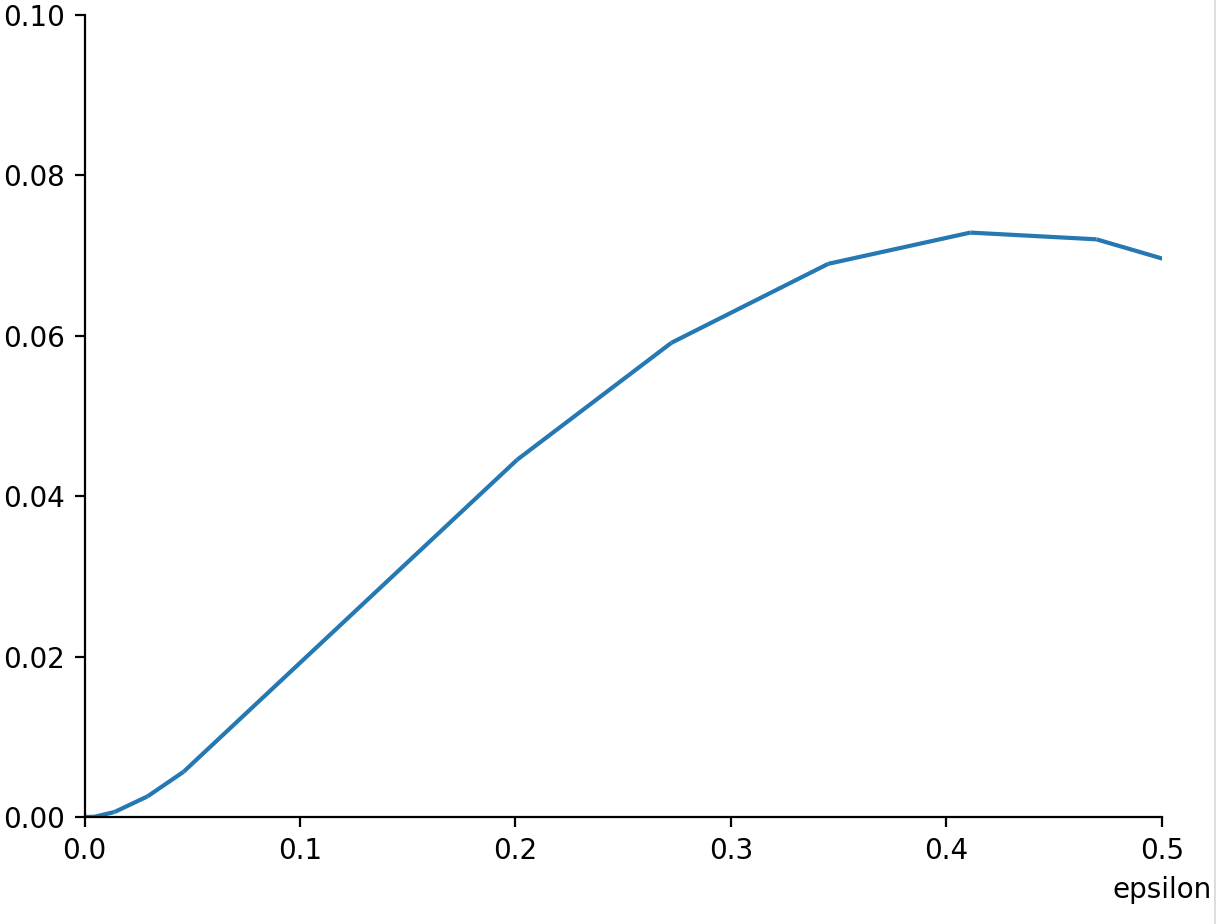
\includegraphics{mult_frac_ep}	
	}
	\caption{The fraction of agents with more than one stable match as a function of $\epsilon$}
	\label{fig:multi_match}
\end{figure}

\subsection{Rank List Length}

\begin{prop}
	Agents are indiferent between submitting a three-entry rank list and their complete preferences.
\end{prop}

\begin{proof}
	As we partition the market as in subsection \ref{subsect:partition}, there is never a case where two people in the same partition have numbers that differ by more than one. Therefore, the partitions and resultant matching are the same if each person submits a 3-member rank list consisting of only agents they might share a partition with.
\end{proof}





\bibliographystyle{aea}
\bibliography{../../library}

% The appendix command is issued once, prior to all appendices, if any.
\appendix



\section{ Appendix}

\subsection{Deferred Acceptance}
The deferred acceptance mechanism is a mainstay of this paper. In the man-proposing version of this mechanism, the algorithm iteritavely selects a man $m$ who proposes to his most preferred woman who has not yet rejected him, unless he has been rejected by all women who he prefers to being unmatched.  If she prefers him to her current tenative assignment (and prefers him to being unmatched), she holds his proposal and rejects her current assignment (if one exists). Otherwise, she rejects $m$.  This process repeats until all men are either tentatively matched or have run out of proposals to make, and arrives at a stable matching that is weakly preferred by all men to any other stable matching.  We call this the man-optimal stable match, because it is weakly preferred by all men to any other stable match.  A parallel result exists for the woman-proposing algorithm.


\subsection{Permutations of preferences for $\{m_1,m_2,w_1,w_2\}$}
I denote preferences with a four-bit binary number, in which a zero in the first position indicates that $w_1\succ_{m_1} w_2$ while a one in the first position indicates that $w_1\prec_{m_1} w_2$. Likewise the second through fourth positions indicate the preferences of $m_2, ,w_1$,and $w_2$.
\\
Type A

$(0,0,0,0)$: $C_0 =\{m_1,w_1\}, \{\phi_0\}=\{m_1,w_1\}$.  Preferences for $\{m_2,m_3,w_2,w_3\}$ are unrestricted.
\\

Type B

$(0,0,1,0)$: $C_0 =\{m_2,w_1\}, \{\phi_0\}=\{m_2,w_1\}, C_1 =\{m_1,w_2\}, \{\phi_1\}=\{m_1,w_2\}$.  Preferences for $\{m_3,m_4,w_3,w_4\}$ are unrestricted.


$(0,0,1,1)$: $C_0 =\{m_2,w_1\}, \{\phi_0\}=\{m_2,w_1\}, C_1 =\{m_1,w_2\}, \{\phi_1\}=\{m_1,w_2\}$.  Preferences for $\{m_3,m_4,w_3,w_4\}$ are unrestricted.


$(0,1,0,1)$: $C_0 =\{m_1,w_1\}, \{\phi_0\}=\{m_1,w_1\}, C_1 =\{m_2,w_2\}, \{\phi_1\}=\{m_2,w_2\}$.  Preferences for $\{m_3,m_4,w_3,w_4\}$ are unrestricted.


$(0,1,1,1)$: $C_0 =\{m_2,w_2\}, \{\phi_0\}=\{m_2,w_2\}, C_1 =\{m_1,w_1\}, \{\phi_1\}=\{m_1,w_1\}$.  Preferences for $\{m_3,m_4,w_3,w_4\}$ are unrestricted.


$(1,0,0,0)$: $C_0 =\{m_1,w_2\}, \{\phi_0\}=\{m_1,w_2\}, C_1 =\{m_2,w_1\}, \{\phi_1\}=\{m_2,w_1\}$.  Preferences for $\{m_3,m_4,w_3,w_4\}$ are unrestricted.


$(1,0,1,0)$: $C_0 =\{m_1,w_2\}, \{\phi_0\}=\{m_1,w_2\}, C_1 =\{m_2,w_1\}, \{\phi_1\}=\{m_2,w_1\}$.  Preferences for $\{m_3,m_4,w_3,w_4\}$ are unrestricted.


$(1,0,1,1)$: $C_0 =\{m_2,w_1\}, \{\phi_0\}=\{m_2,w_1\}, C_1 =\{m_1,w_2\}, \{\phi_1\}=\{m_1,w_2\}$.  Preferences for $\{m_3,m_4,w_3,w_4\}$ are unrestricted.



$(1,1,0,0)$:  $C_0 =\{m_1,w_2\}, \{\phi_0\}=\{m_1,w_2\}, C_1 =\{m_2,w_1\}, \{\phi_1\}=\{m_2,w_1\}$.  Preferences for $\{m_3,m_4,w_3,w_4\}$ are unrestricted.


$(1,1,0,1)$:  $C_0 =\{m_2,w_2\}, \{\phi_0\}=\{m_2,w_2\}, C_1 =\{m_1,w_1\}, \{\phi_1\}=\{m_1,w_1\}$.  Preferences for $\{m_3,m_4,w_3,w_4\}$ are unrestricted.



$(1,1,1,0)$:  $C_0 =\{m_1,w_2\}, \{\phi_0\}=\{m_1,w_2\}, C_1 =\{m_2,w_1\}, \{\phi_1\}=\{m_2,w_1\}$.  Preferences for $\{m_3,m_4,w_3,w_4\}$ are unrestricted.



$(1,1,1,1)$:  $C_0 =\{m_2,w_2\}, \{\phi_0\}=\{m_2,w_2\}, C_1 =\{m_1,w_1\}, \{\phi_1\}=\{m_1,w_1\}$.  Preferences for $\{m_3,m_4,w_3,w_4\}$ are unrestricted.
\\

Type C

$(1,0,0,1)$:  $C_0 =\{m_1,w_1,m_2,w_2\}$ or $C_0 =\{m_1,w_1,m_2,w_2, w_3\}$ if $w_3\succ_{m_2} w_2$, $\{\phi_0\}=\{m_1,w_1,m_2,w_2\}$.  Preferences for $\{m_3,m_4,w_3,w_4\}$ are unrestricted. 

$(0,1,1,0)$:  $C_0 =\{m_1,w_1,m_2,w_2\}$ or $C_0 =\{m_1,w_1,m_2,w_2, m_3\}$ if $m_3\succ_{w_2} m_2$, $\{\phi_0\}=\{m_1,w_1,m_2,w_2\}$.  Preferences for $\{m_3,m_4,w_3,w_4\}$ are unrestricted. 
\\


Type D

$(0,0,0,1)$:  $C_0 =\{m_1,w_1\}, \{\phi_0\}=\{m_1,w_1\}$.  Preferences for $\{m_2,m_3,w_2,w_3\}$ fit the pattern $(\cdot,\cdot,0,\cdot)$.


$(0,1,0,0)$:  $C_0 =\{m_1,w_1\}, \{\phi_0\}=\{m_1,w_1\}$.  Preferences for $\{m_2,m_3,w_2,w_3\}$ fit the pattern $(0,\cdot,\cdot,\cdot)$.



\end{document}

